\documentclass{article}

% Language setting
% Replace `english' with e.g. `spanish' to change the document language
\usepackage[english]{babel}

% Custom packages
\usepackage{color,soul} % For highlighting text
\usepackage{float} % For controlling figure placement ([H] option)
\usepackage{amsmath}
\usepackage{amssymb} % For mathematical symbols such as \lessgtr
\DeclareMathOperator*{\argmax}{arg\,max}
\DeclareMathOperator*{\argmin}{arg\,min}

% Set page size and margins
% Replace `letterpaper' with `a4paper' for UK/EU standard size
\usepackage[letterpaper,top=2cm,bottom=2cm,left=3cm,right=3cm,marginparwidth=1.75cm]{geometry}

% Useful packages
\usepackage{graphicx}
\usepackage[colorlinks=true, allcolors=blue]{hyperref}

\newcommand{\mi}{\mathrm{i}}

\title{Statistical analysis of Kernel-Nulling output distributions for high contrast detection of exoplanets in VLTI and LIFE configurations}

\author{Vincent Foriel,
        David Mary,
        Frantz Martinache
       }

\begin{document}

\maketitle

\begin{abstract}
Kernel-nulling interferometry represents a promising approach for direct exoplanet detection. This technique generates characteristic kernel-null depth distributions depending on the presence or absence of a planetary companion. Statistical analysis of these distributions is essential for robust planet detection. We develop and compare several statistical tests to efficiently discriminate between the H0 (star-only) and H1 (star-planet system) hypotheses. We analyze the performance of different test statistics including mean, median, argmax, Kolmogorov-Smirnov, Cramér-von Mises, and Wilcoxon-Mann-Whitney tests. We conduct numerical simulations for two instrumental scenarios: ground-based VLTI and space-based LIFE configurations. For each scenario, we generate datasets under both H0 and H1 hypotheses, accounting for specific instrumental parameters and noise levels. We evaluate test performance using ROC curves and P-value analysis. \hl{Ajouter les résultats}. This statistical analysis, currently applied to simulated data, paves the way for robust high-contrast exoplanet detection using kernel-nulling interferometry.
\end{abstract}

%------------------------------------------------------------------------------

\section{Introduction}

Direct imaging of exoplanets remains one of the major challenges in modern astronomy, requiring techniques capable of overcoming contrast constraints (beyond $10^{-8}$ to allow exo-Earth detection) and angular separation requirements (on the order of milli-arcseconds). Nulling interferometry, initially proposed by \cite{Bracewell1979}, uses destructive interference to suppress stellar light while preserving the planetary signal, thus addressing both angular resolution and contrast challenges.

Kernel-Nulling \cite{Martinache2018} improves this approach by using four telescopes and phase-quadrature signals, enabling the creation of signal combinations (Kernel-Nulls) that are robust to first-order phase aberrations. This technique generates characteristic statistical distributions depending on the presence or absence of a planetary companion (Fig \ref{fig:distribution}). However, these distributions do not follow conventional probability laws (discussed in Sec. \ref{sec:distribution_analysis}).

Analysis of these distributions therefore requires appropriate statistical tools to efficiently discriminate between the two hypotheses: H0 (star-only) and H1 (star-planet system). In this work, we develop and compare several statistical tests to optimize exoplanet detection using Kernel-Nulling.

\begin{figure}[H]
\centering
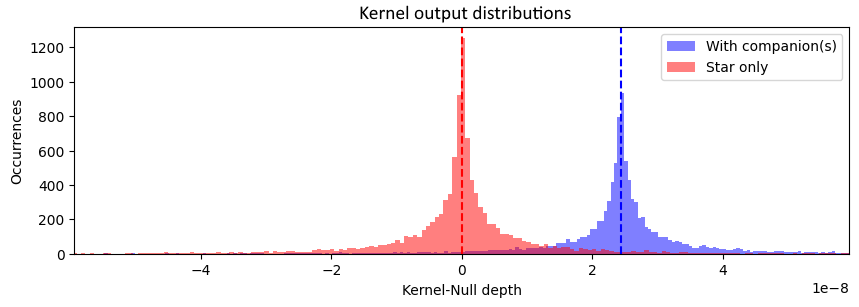
\includegraphics[width=\linewidth]{img/output_distribution.png}
\caption{Example of kernel-null depth distributions for H0 (star-only) and H1 (with companion) hypotheses. This example scenario is highly exagerated with a companion that has low contrast in order to induce a significant shift of the distribution. In practice, the two distributions are usually much closer and hard to distinguish.}
\label{fig:distribution}
\end{figure}

%--------------------------------------------------------------------

\section{Methodology}

\subsection{Data generation}

In this study, we consider two distinct instrumental scenarios for generating simulated data:

\begin{table}[H]
\centering
\begin{tabular}{|l|c|c|}
\hline
\textbf{Parameter} & \textbf{VLTI} & \textbf{LIFE} \\
\hline
Number of telescopes & 4 & 4 \\
Telescope diameter & 8 m & 2 m \\
Configuration & Irregular & Regular (rectangular) \\
Maximum baseline & 130 m & 600 m \\
Operating environment & Ground & Space \\
Wavelength & $1.55\mu$m & $4\mu$m \\
Cophasing error (RMS) & 100 nm & 1 nm \\
\hline
\end{tabular}
\caption{Instrumental parameters for the two scenarios considered in this study.}
\label{tab:scenarios}
\end{table}

The VLTI scenario includes residual cophasing error of 100 nm RMS, representative of atmospheric conditions and phase control system limitations at VLTI. The LIFE scenario benefits from the space environment, allowing a reduction of the cophasing error to 1 nm RMS, reflecting the increased stability expected for a space mission such as LIFE.

For each scenario, datasets are generated under both H0 (star-only) and H1 (star-planet system) hypotheses, accounting for specific instrumental parameters and noise levels for each case. The Kernel-Nulling operation is supposed ideal.

\subsection{Distribution analysis}  \label{sec:distribution_analysis}

Before attempting to discriminate between the H0 and H1 hypotheses, it is essential to study the obtained distributions to identify characteristics that might facilitate their analysis. For this purpose, we compare simulated distributions to different conventional probability laws, notably observing their symmetry and general shape.

We find that no conventional law perfectly matches the observed distributions. Among the tested laws, the Cauchy distribution seems to offer a relatively satisfactory fit (Fig. \ref{fig:fits}), although not perfect, especially on the wings when the number of sample is high.

This observation guides the choice of statistical tests to favor, particularly those effective for detecting shifts in symmetric distributions. Furthermore, this suggests that data fitting by minimizing square error (MSE) will most likely not be very effective due to the heavy tails of the distribution. Instead, we should use a cost function derived from the Cauchy law, which is more robust to outliers:
\begin{equation}
    \text{Cost}(x, y) = \sum_i \log \left( 1 + \left( y_i - s(x_i )\right)^2 \right)
\end{equation}

\begin{figure}[H]
\centering
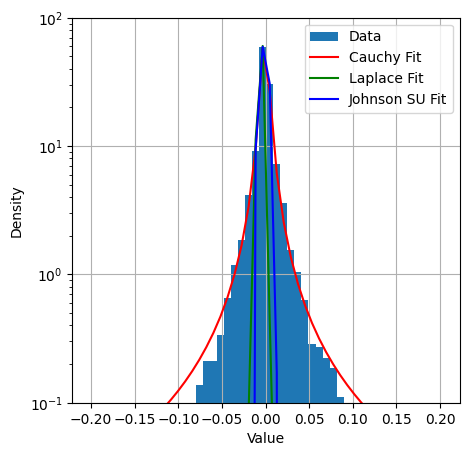
\includegraphics[width=6cm]{img/fits.png}
\caption{Fitting of conventional probability laws to simulated distributions.The Fitter python package was used to perform the fitting of most of the usual laws. This figure show the fit of the three most relevant laws the package pointed out.}
\label{fig:fits}
\end{figure}

\subsection{Statistical tests implemented}

We have developed and compared several test statistics:

\subsubsection{Mean}

The test statistic based on the mean compares the absolute value of the distribution mean to a threshold:

\begin{equation}
    \left|\frac{1}{N}\sum_i x_i \right| \stackrel{H_1}{\underset{H_0}{\gtrless}} \xi
\end{equation}

\subsubsection{Median}
Test based on the absolute value of the distribution median.

\begin{equation}
\begin{cases}
\left| x_{\frac{N+1}{2}} \right| & \text{if }N\text{ is odd} \\
\left| \frac{x_{\frac{N}{2}} + x_{\frac{N+1}{2}}}{2} \right|  & \text{if }N\text{ is even}
\end{cases}
\quad\stackrel{H_1}{\underset{H_0}{\gtrless}} \xi
\end{equation}

\subsubsection{Argmax}
This statistic examines the position of the bin with the highest number of occurrences in the data histogram.

\hl{Décrire formèlement}

\subsubsection{Kolmogorov-Smirnov}
Test comparing the maximum distance between the cumulative distribution functions of the two distributions.

\hl{Décrire formèlement}

\subsubsection{Cramér-von Mises}
Test based on the total quadratic distance between cumulative distribution functions.

\hl{Décrire formèlement}

\subsubsection{Wilcoxon-Mann-Whitney}
Non-parametric test for comparing two independent samples.

\hl{Décrire formèlement}

\subsubsection{CDF difference area}
This statistic measures the area between the cumulative distribution functions of the two distributions.

\hl{Décrire formèlement}

%--------------------------------------------------------------------

\section{Results}

\subsection{ROC curves}

ROC (Receiver Operating Characteristic) curves allow comparing the effectiveness of different test statistics by representing the proportion of true detections as a function of false alarm probability.

\begin{figure}[H]
\centering
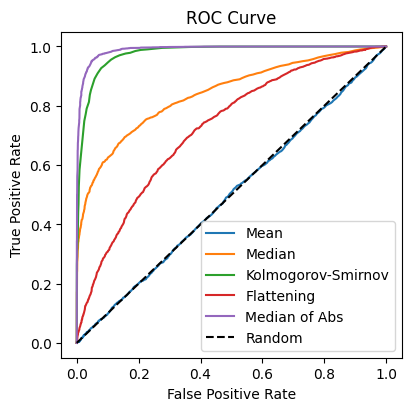
\includegraphics[width=7cm]{img/roc_curves.png}
\caption{ROC curves for different test statistics.}
\label{fig:roc}
\end{figure}

\hl{Analyse des résultats}
\hl{Ajouter la courbe de Neyman-Pearson pour la comparaison}

\subsection{P-value analysis}

P-values provide a confidence measure for rejecting the null hypothesis. A P-value below 0.05 is generally considered significant.

\begin{figure}[H]
\centering
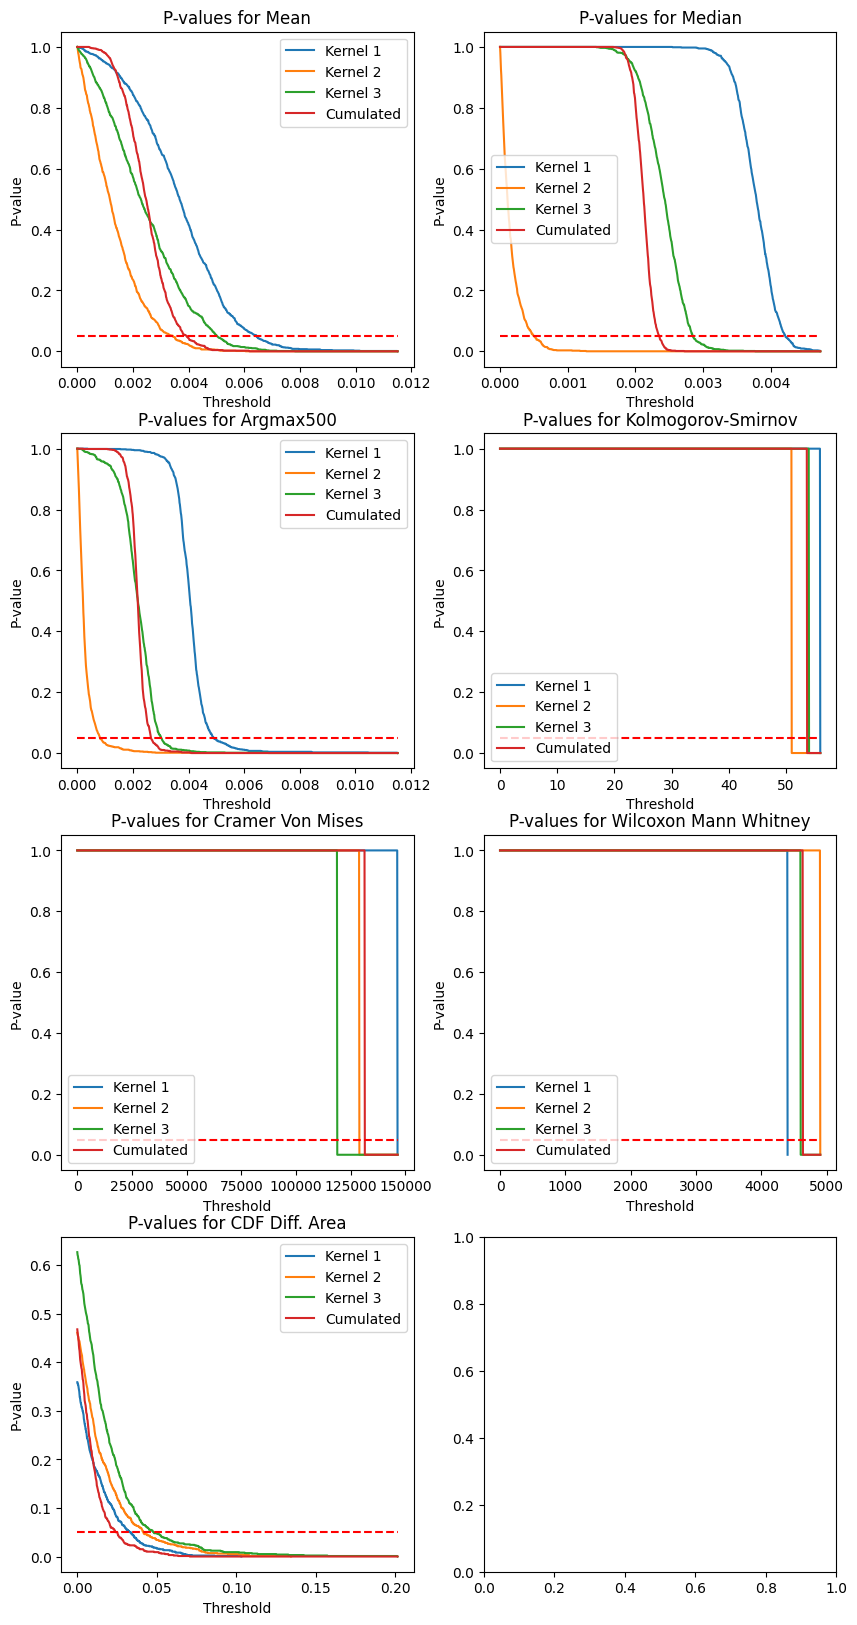
\includegraphics[width=10cm]{img/p-values.png}
\caption{Evolution of P-values as a function of threshold for different test statistics. The red dotted line indicates the significance threshold at 0.05. \hl{Plot à refaire pour se focaliser sur un seul Kernel (+ correction des bugs)}}
\label{fig:pvalues}
\end{figure}

\hl{Analyse des résultats}

%--------------------------------------------------------------------

\section{Discussion}

\subsection{Comparative test performance}

\hl{ToDo}

\subsection{Noise sensitivity}

\hl{ToDo}


%-----------------------------------------------------------------

\section{Conclusions}

\hl{ToDo}

\bibliographystyle{alpha}
\bibliography{sample}

\end{document}